\documentclass[usenames,dvipsnames]{beamer}

%\usepackage{default}
\usepackage{tikz}
\usetikzlibrary{backgrounds}
\usetikzlibrary{arrows}

\usepackage{algorithm}
\usepackage{algpseudocode}
\usepackage{algorithmicx}

\usetheme{Berlin}

\renewcommand{\.}{. \;}
\theoremstyle{definition}
\newtheorem*{definition}{Definition}
\newtheorem*{example}{Example}

\theoremstyle{plain}
\newtheorem{theorem}{Theorem}

\theoremstyle{remark}
\newtheorem*{remark}{Remark}

\newcommand{\pto}{\nrightarrow}
\newcommand{\ptree}[3]{
	\ifx&#2&%
	(#1 \rightrightarrows #3)
	\else
	(#1^#2 \rightrightarrows #3)
	\fi
}

\newcommand{\allgraphs}[1]{\mathcal{G}_{#1}}
\newcommand{\alltgraphs}[1]{\mathcal{TG}_{#1}}
\newcommand{\emptyGraph}{\varepsilon}
\newcommand{\startG}[1]{Z_{#1}}
\newcommand{\startTG}[1]{Z_{#1}}
\newcommand{\pro}{\to}

\newcommand{\rel}{\sim}
\newcommand{\rrestr}{\triangleright}

\newcommand{\source}{\operatorname{s}}
\newcommand{\Source}{\operatorname{S}}
\newcommand{\target}{\operatorname{t}}
\newcommand{\Target}{\operatorname{T}}


\newcommand{\neigh}[1]{\operatorname{neigh}_{#1}}
\newcommand{\scont}[2]{\eta_{#1}(#2)}
\newcommand{\cont}[2]{\operatorname{cont}_{#1}(#2)}
\newcommand{\emb}[1]{\operatorname{emb}(#1)}

\newcommand{\st}{\; | \;}
\newcommand{\isomorph}{\cong}
\newcommand{\ms}[1]{\overset{#1}{\leftarrow}}
\newcommand{\mt}[1]{\overset{#1}{\rightarrow}}
\newcommand{\cderiv}[3]{
	\ifx&#2&%
	\overset{#1}{\Rrightarrow}_{#3}
	\else
	\overset{#1,#2}{\Rrightarrow}_{#3}
	\fi
}
\newcommand{\deriv}[3]{
	\ifx&#2&%
	\overset{#1}{\Rightarrow}_{#3}
	\else
	\overset{#1,#2}{\Rightarrow}_{#3}
	\fi
}
\newcommand{\derivtr}[3]{
	\ifx&#2&%
	\overset{#1}{\Rightarrow^*}_{#3}
	\else
	\overset{#1,#2}{\Rightarrow^*}_{#3}
	\fi
}
\newcommand{\tcderiv}[3]{
	\ifx&#2&%
	\overset{#1}{\Rrightarrow}_{#3}
	\else
	\overset{#1,#2}{\Rrightarrow}_{#3}
	\fi
}
\newcommand{\tderiv}[3]{
	\ifx&#2&%
	\overset{#1}{\Rightarrow}_{#3}
	\else
	\overset{#1,#2}{\Rightarrow}_{#3}
	\fi
}
\newcommand{\tderivtr}[3]{
	\ifx&#2&%
	\overset{#1}{\Rightarrow^*}_{#3}
	\else
	\overset{#1,#2}{\Rightarrow^*}_{#3}
	\fi
}

\newcommand{\?}{\operatorname{\textbf{?}}}
\renewcommand{\:}{\operatorname{\textbf{:}}}
\newcommand{\Break}{\textbf{break}}

\tikzstyle{grammar}=[shorten >=1pt,->,draw=black!50]
\tikzstyle{graph}=[shorten >=1pt,->,draw=black!50]
\tikzstyle{rid} = [align=left, anchor=east]
\tikzstyle{nont}=[rectangle,inner sep=5pt, draw, fill=white, minimum width=20pt]
\tikzstyle{t}=[circle,inner sep=3pt, draw, fill=white, minimum width=15pt]
\tikzstyle{g}=[inner sep=3pt, fill=white]
\tikzstyle{lhs}=[inner sep=5pt, fill=white]
\tikzstyle{w}=[circle, inner sep=2pt, below=8pt, draw, fill=white]
\tikzstyle{edge}=[->, very thick, -latex]
\tikzstyle{edgeLabel}=[midway, above]
\tikzstyle{wedge}=[-, thick]
\tikzstyle{biedge}=[-, very thick]
\tikzstyle{pipe}=[-, very thick]
\tikzstyle{morph}=[-, very thick, dashed, -latex]


\usepackage{appendixnumberbeamer}

%Header Settings
\setbeamertemplate{headline}{}

%Footer Settings
\setbeamertemplate{navigation symbols}{
	\usebeamerfont{footline}%
	\usebeamercolor[fg]{footline}%
	\hspace{1em}%
	\insertframenumber/\inserttotalframenumber
}

\title[Transformations with TGG with Non-terminal Symbols]{Transformations with Triple Graph Grammars with Non-terminal Symbols}
\author[W. da Silva et al.]{William da Silva, Max Bureck, Ina Schieferdecker, and Christian Hein}
\institute[Fraunhofer Fokus]
{
	\vskip 12pt
	Fraunhofer Fokus, Berlin, Germany \\
	\texttt{william.bombardelli.da.silva@fokus.fraunhofer.de}\\
	Technische Universit\"{a}t Berlin, Berlin, Germany
}
\date{December 5, 2018}

\makeatletter
\hypersetup{
	pdftitle = {\@title}, pdfkeywords = {Model Transformation}, pdfauthor = {\@author}
} 
\makeatother

\begin{document}
	\begin{frame}
		\titlepage
	\end{frame}
	
	\begin{frame}
		\frametitle{Organization}
		\tableofcontents
	\end{frame}
	
	%-------------------
	% Introduction
	%-------------------
	\section{Introduction}
	\begin{frame}
		\frametitle{Introduction}
		\tableofcontents[currentsection, currentsubsection] 
	\end{frame}
	
	\begin{frame}{Background}
		\begin{itemize}
			\item Model-driven software development as a technique to enhance quality of software
			\pause
			\item Models as formal specifications of safety-critical systems
			\pause
			\item Transformation between models (e.g. from a formal specification to high-level source-code and vice-versa)
			\pause
			\medskip
			\item \textbf{Goal:} Comprehensible and reliable transformations
			\begin{itemize}
				\item Efficient representation of abstract concepts
				\item Small size
			\end{itemize}
		\end{itemize}
	\end{frame}
	
	\begin{frame}{The Model Transformation Problem}
		\centering{
		\includegraphics[width=.7\textwidth]{misc/model-transformation}
		}
		\begin{itemize}
			\item $G \ct T$ iff $G$ is correctly transformed into $T$
			\item $\ct$ is the \emph{correctly-transformed relation} between source and target models
			\item \textbf{Batch forward transformation:} \\
			Given $G$, find a $T$, such that $G \ct T$
		\end{itemize}
	\end{frame}
	
	\begin{frame}{The Triple Graph Grammar Approach}
		\begin{itemize}
			\item Models are graphs
			\pause
			\item Two correctly-transformed graphs $G$ and $T$ are in a triple graph $G \ms{} C \mt{} T$\\
				\begin{tikzpicture}[graph]
	\draw (1,0) node[t] (s1) {cd};
	\draw (1,-1.5) node[t] (s2) {c};
	\draw (2,-1.5) node[t] (s4) {a};
	\draw (2,0) node[t] (s5) {c};
	\draw[edge] (s1) -- (s2) node [vledgeLabel] {$\kappa$};
	\draw[edge] (s1) -- (s4) node [vredgeLabel] {$\alpha$};
	\draw[edge] (s1) -- (s5) node [edgeLabel, below] {$\kappa$};
	\draw[edge] (s4) -- (s2) node [edgeLabel] {$\zeta$};
	\draw[edge] (s4) -- (s5) node [vredgeLabel] {$\psi$};
	%
	\draw (3,0.5) node[t] (c1) {dd};
	\draw (3,-2) node[t] (c2) {ct};
	\draw (3,-1.5) node[t] (c4) {ac};
	\draw (3,-0.5) node[t] (c5) {ct};
	%
	\draw (5,0) node[t] (t1) {db};
	\draw (5,-1.5) node[t] (t2) {t};
	\draw (4,-1.5) node[t] (t4) {co};
	\draw (4,0) node[t] (t5) {t};
	\draw[edge] (t1) -- (t2) node [vredgeLabel] {$\pi$};
	\draw[edge] (t1) -- (t5) node [edgeLabel, below] {$\pi$};
	\draw[edge] (t2) -- (t4) node [edgeLabel] {$\gamma$};
	\draw[edge] (t4) -- (t5) node [vledgeLabel] {$\delta$};
	%
	\draw[morph] (c1) -- (s1);
	\draw[morph] (c1) -- (t1);
	\draw[morph] (c2) -- (s2);
	\draw[morph] (c2) -- (t2);
	\draw[morph] (c4) -- (s4);
	\draw[morph] (c4) -- (t4);
	\draw[morph] (c5) -- (s5);
	\draw[morph] (c5) -- (t5);
	\end{tikzpicture}

			\pause
			\item A triple graph grammar $TGG$ is a generator of a set of triple graphs $L(TGG)$
			\pause
			\item The correctly-transformed relation $\ct$ between graphs is described in terms of a triple graph grammar $TGG$
			\begin{itemize}
				\item $G \ct T $ iff $(G \ms{} C \mt{} T) \in L(TGG)$
			\end{itemize}
		\end{itemize}
	\end{frame}
	
	\begin{frame}{TGG -- An Example}
		\begin{itemize}
			\item \emph{Pseudocode} to \emph{Controlflow}
		\end{itemize}
		
		\begin{figure}
\footnotesize{
\begin{minipage}[h]{.3\textwidth}
	\begin{algorithmic}[!ht]
		\State \Program $main(n)$
		\If {$n < 0$}
			\State \Return $\Nothing$
		\Else
			\State $f \gets 1$ 
			\While {$n > 0$}
				\State $f \gets f * n$
				\State $n \gets n - 1$
			\EndWhile
			\State \Return $\Just f$
		\EndIf
	\end{algorithmic}
\end{minipage}
\begin{minipage}[h]{.5\textwidth}
	\begin{tikzpicture}[graph]
	\draw (1,0) node[t] (s1) {p};
	\draw (1,-0.7) node[t] (s2) {i};
	\draw (1.5,-1.3) node[t] (s3) {a};
	\draw (0.5,-1.4) node[t] (s4) {a};
	\draw (0.5,-2.1) node[t] (s5) {w};
	\draw (0.5,-2.8) node[t] (s6) {a};
	\draw (0.5,-3.5) node[t] (s7) {a};
	\draw (0.5,-4.2) node[t] (s8) {a};
	
	\draw[edge] (s1) -- (s2) node [vledgeLabel] {$f$};
	\draw[edge] (s2) -- (s3) node [vredgeLabel] {$p$};
	\draw[edge] (s2) -- (s4) node [vledgeLabel] {$n$};
	\draw[edge] (s4) -- (s5) node [vledgeLabel] {$x$};
	\draw[edge] (s5) -- (s6) node [vledgeLabel] {$f$};
	\draw[edge] (s5) to [bend left] (s7) node [above=25pt, right=3pt] {$l$};
	\draw[edge] (s5) to [bend right=60] (s8) node [above=30pt, left=13pt] {$x$};
	\draw[edge] (s6) -- (s7) node [vledgeLabel] {$x$};
	%
	\draw (3,0) node[t] (c1) {pg};
	\draw (3,-0.5) node[t] (c2) {ib};
	\draw (3,-1.0) node[t] (c3) {ac};
	\draw (3,-1.8) node[t] (c4) {ac};
	\draw (3,-2.3) node[t] (c5) {wb};
	\draw (3,-2.8) node[t] (c6) {ac};
	\draw (3,-3.5) node[t] (c7) {ac};
	\draw (3,-4.2) node[t] (c8) {ac};
	%
	\draw (5,0) node[t] (t1) {g};
	\draw (5,-0.7) node[t] (t2) {b};
	\draw (5.5,-1.3) node[t] (t3) {c};
	\draw (4.5,-1.5) node[t] (t4) {c};
	\draw (4.5,-2.1) node[t] (t5) {b};
	\draw (4.5,-2.8) node[t] (t6) {c};
	\draw (4.5,-3.5) node[t] (t7) {c};
	\draw (4.5,-4.2) node[t] (t8) {c};
	
	\draw[edge] (t1) -- (t2) node [vledgeLabel] {$r$};
	\draw[edge] (t2) -- (t3) node [vredgeLabel] {$p$};
	\draw[edge] (t2) -- (t4) node [above=15pt, right=0pt] {$n$};
	\draw[edge] (t4) -- (t5) node [vledgeLabel] {$x$};
	\draw[edge] (t5) -- (t6) node [vledgeLabel] {$f$};
	\draw[edge] (t7) to [bend right] (t5) node [below=15pt, right=3pt] {$x$};
	\draw[edge] (t5) to [bend right=60] (t8) node [above=30pt, left=13pt] {$x$};
	\draw[edge] (t6) -- (t7) node [vledgeLabel] {$x$};
	%
	\draw[morph] (c1) -- (s1);
	\draw[morph] (c1) -- (t1);
	\draw[morph] (c2) -- (s2);
	\draw[morph] (c2) -- (t2);
	\draw[morph] (c3) -- (s3);
	\draw[morph] (c3) -- (t3);
	\draw[morph] (c4) -- (s4);
	\draw[morph] (c4) -- (t4);
	\draw[morph] (c5) -- (s5);
	\draw[morph] (c5) -- (t5);
	\draw[morph] (c6) -- (s6);
	\draw[morph] (c6) -- (t6);
	\draw[morph] (c7) -- (s7);
	\draw[morph] (c7) -- (t7);
	\draw[morph] (c8) -- (s8);
	\draw[morph] (c8) -- (t8);
	\end{tikzpicture}
\end{minipage}
}
\end{figure}

	\end{frame}
	
	\begin{frame}{TGG -- An Example}
		\begin{itemize}
			\item \emph{Pseudocode} to \emph{Controlflow}
		\end{itemize}
			
			\centering
	\begin{tikzpicture}[grammar]
	\node[rid] at (\ridX,\ridY) {$r_0:$};
	\draw (\lhsX,0) node[lhs] (lhs) {::=};
	
	\draw (0.5,0) node[t] (s1) {p};
	%%
	\draw (1.5,0) node[t] (c1) {pg};
	%%
	\draw (2.5,0) node[t] (t1) {g};
	%%
	\draw[morph] (c1) -- (s1);
	\draw[morph] (c1) -- (t1);
	\end{tikzpicture}
		
	\vskip 5pt
		
	\begin{tikzpicture}[grammar]
	\node[rid] at (\ridX,\ridY) {$r_1:$};
	
	\draw (0,0) node[t] (s1) {p};
	%%
	\draw (1,0) node[t] (c1) {pg};
	%%
	\draw (2,0) node[t] (t1) {g};
	%%
	\draw[morph] (c1) -- (s1);
	\draw[morph] (c1) -- (t1);
	%%%%%%
	\draw (3,0) node[lhs] (lhs) {::=};
	%%%%%%	
	\draw (4,0) node[t] (s2) {p};
	\draw (4,-1) node[t] (s3) {a};
	\draw[edge] (s2) -- (s3) node [vledgeLabel] {$f$};
	%%
	\draw (5,0) node[t] (c2) {pg};
	\draw (5,-1) node[t] (c3) {ac};
	%%
	\draw (6,0) node[t] (t2) {g};
	\draw (6,-1) node[t] (t3) {c};
	\draw[edge] (t2) -- (t3) node [vledgeLabel] {$r$};
	%%
	\draw[morph] (c1) -- (s1);
	\draw[morph] (c1) -- (t1);
	\draw[morph] (c2) -- (s2);
	\draw[morph] (c2) -- (t2);
	\draw[morph] (c3) -- (s3);
	\draw[morph] (c3) -- (t3);
	\end{tikzpicture}
	
	\vskip 5pt
	
	\begin{tikzpicture}[grammar]
	\node[rid] at (\ridX,\ridY) {$r_2:$};
	
	\draw (0,0) node[t] (s1) {i};
	%%
	\draw (1,0) node[t] (c1) {ib};
	%%
	\draw (2,0) node[t] (t1) {b};
	%%
	\draw[morph] (c1) -- (s1);
	\draw[morph] (c1) -- (t1);
	%%%%%%
	\draw (3,0) node[lhs] (lhs) {::=};
	%%%%%%
	\draw (5,0) node[t] (s2) {i};
	\draw (4,-1) node[t] (s3) {a};
	\draw (5,-1.2) node[t] (s4) {a};
	\draw (6,-1) node[t] (s5) {a};
	\draw[edge] (s2) -- (s3) node [vledgeLabel] {$x$};
	\draw[edge] (s2) -- (s4) node [vledgeLabel] {$p$};
	\draw[edge] (s2) -- (s5) node [vredgeLabel] {$n$};
	%%
	\draw (7,0) node[t] (c2) {ib};
	\draw (7,-0.5) node[t] (c3) {ac};
	\draw (7,-1.5) node[t] (c4) {ac};
	\draw (7,-1) node[t] (c5) {ac};
	%%
	\draw (9,0) node[t] (t2) {b};
	\draw (10,-1) node[t] (t3) {c};
	\draw (9,-1.2) node[t] (t4) {c};
	\draw (8,-1) node[t] (t5) {c};
	\draw[edge] (t2) -- (t3) node [vledgeLabel] {$x$};
	\draw[edge] (t2) -- (t4) node [vledgeLabel] {$p$};
	\draw[edge] (t2) -- (t5) node [vledgeLabel] {$n$};
	%%
	\draw[morph] (c1) -- (s1);
	\draw[morph] (c1) -- (t1);
	\draw[morph] (c2) -- (s2);
	\draw[morph] (c2) -- (t2);
	\draw[morph] (c3) -- (s3);
	\draw[morph] (c3) -- (t3);
	\draw[morph] (c4) -- (s4);
	\draw[morph] (c4) -- (t4);
	\draw[morph] (c5) -- (s5);
	\draw[morph] (c5) -- (t5);
	\end{tikzpicture}
	\end{frame}
	
	\begin{frame}{TGG -- Derivation}
		\centering
	$\tderiv{r_0}{}{}$
	\begin{tikzpicture}[graph]
	\draw (0.5,0) node[t] (s1) {p};
	\draw (1.5,0) node[t] (c1) {pg};
	\draw (2.5,0) node[t] (t1) {g};
	%%
	\draw[morph] (c1) -- (s1);
	\draw[morph] (c1) -- (t1);
	\end{tikzpicture}
	\pause
	$\tderiv{r_1}{}{}$
	\begin{tikzpicture}[graph]
	\draw (4,0) node[t] (s2) {p};
	\draw (4,-1) node[t] (s3) {i};
	\draw[edge] (s2) -- (s3) node [vledgeLabel] {$f$};
	%%
	\draw (5,0) node[t] (c2) {pg};
	\draw (5,-1) node[t] (c3) {ib};
	%%
	\draw (6,0) node[t] (t2) {g};
	\draw (6,-1) node[t] (t3) {b};
	\draw[edge] (t2) -- (t3) node [vledgeLabel] {$r$};
	%%
	\draw[morph] (c2) -- (s2);
	\draw[morph] (c2) -- (t2);
	\draw[morph] (c3) -- (s3);
	\draw[morph] (c3) -- (t3);
	\end{tikzpicture}
	\pause
	
	\vskip 20pt
	
	$\tderiv{r_2}{}{}$
	\begin{tikzpicture}[graph]
	\draw (5,1) node[t] (s1) {p};
	\draw (5,0) node[t] (s2) {i};
	\draw (4,-1) node[t] (s3) {a};
	\draw (5,-1.2) node[t] (s4) {a};
	\draw (6,-1) node[t] (s5) {a};
	\draw[edge] (s1) -- (s2) node [vledgeLabel] {$f$};
	\draw[edge] (s2) -- (s3) node [vledgeLabel] {$x$};
	\draw[edge] (s2) -- (s4) node [vledgeLabel] {$p$};
	\draw[edge] (s2) -- (s5) node [vredgeLabel] {$n$};
	%%
	\draw (7,1) node[t] (c1) {pg};
	\draw (7,0) node[t] (c2) {ib};
	\draw (7,-0.5) node[t] (c3) {ac};
	\draw (7,-1.5) node[t] (c4) {ac};
	\draw (7,-1) node[t] (c5) {ac};
	%%
	\draw (9,1) node[t] (t1) {g};
	\draw (9,0) node[t] (t2) {b};
	\draw (10,-1) node[t] (t3) {c};
	\draw (9,-1.2) node[t] (t4) {c};
	\draw (8,-1) node[t] (t5) {c};
	\draw[edge] (t1) -- (t2) node [vledgeLabel] {$r$};
	\draw[edge] (t2) -- (t3) node [vledgeLabel] {$x$};
	\draw[edge] (t2) -- (t4) node [vledgeLabel] {$p$};
	\draw[edge] (t2) -- (t5) node [vledgeLabel] {$n$};
	%%
	\draw[morph] (c1) -- (s1);
	\draw[morph] (c1) -- (t1);
	\draw[morph] (c2) -- (s2);
	\draw[morph] (c2) -- (t2);
	\draw[morph] (c3) -- (s3);
	\draw[morph] (c3) -- (t3);
	\draw[morph] (c4) -- (s4);
	\draw[morph] (c4) -- (t4);
	\draw[morph] (c5) -- (s5);
	\draw[morph] (c5) -- (t5);
	\end{tikzpicture}

	\end{frame}
	
	%-------------------
	%  TGG With Non-terminals
	%-------------------
	\section{Triple Graph Grammars with Non-terminal Symbols}
	\begin{frame}
		\frametitle{Triple Graph Grammars with Non-terminal Symbols}
		\tableofcontents[currentsection, currentsubsection] 
	\end{frame}
	
	\begin{frame}{Our Contribution -- NCE TGG}
		\begin{itemize}
			\item New formalism: NCE TGG
			\begin{itemize}
				\item \emph{Graph Grammar with Neighborhood-controlled Embedding} (NCE) \cite{janssens1982graph}
				\item \emph{Triple Graph Grammar} (TGG) \cite{schurr1994specification}
			\end{itemize}
			\item Non-terminal symbols
			\item Context-free
		\end{itemize}
	\end{frame}
	
	\begin{frame}{NCE TGG -- An Example}
		\begin{itemize}
			\item \emph{Pseudocode} to \emph{Controlflow}
		\end{itemize}
		
		\begin{example}{Pseudocode to ControlFlow.}
	$GG = (\{S,A,B,a,b,c\}, \{a,b,c\}, S, P)$, where $P$ is

	\noindent
	\begin{tikzpicture}[grammar]
	\node[rid] at (\ridX,\ridY) {$r_0:$};
	\draw (\lhsX,0) node[lhs] (lhs) {S ::=};
	
	\draw (0.5,0) node[t] (s1) {p};
	\draw (0.5,-1) node[nont] (s2) {A};
	\draw[edge] (s1) -- (s2) node [vedgeLabel] {$f$};
	%%
	\draw (2,0) node[t] (c1) {pg};
	\draw (2,-1) node[nont] (c2) {A};
	%%
	\draw (3.5,0) node[t] (t1) {g};
	\draw (3.5,-1) node[nont] (t2) {A};
	\draw[edge] (t1) -- (t2) node [vedgeLabel] {$f$};
	%%
	\draw[morph] (c1) -- (s1);
	\draw[morph] (c1) -- (t1);
	\draw[morph] (c2) -- (s2);
	\draw[morph] (c2) -- (t2);
	\end{tikzpicture}
	\begin{tikzpicture}[grammar]
	\node[rid] at (\ridX,\ridY) {$r_1:$};
	\draw (\lhsX,0) node[lhs] (lhs) {A ::=};
	
	\draw (0.5,0) node[t] (s1) {a};
	\draw (0.5,-1) node[nont] (s2) {A};
	\draw[edge] (s1) -- (s2) node [vedgeLabel] {$x$};
	\draw node[uw, label=0:$f;x;x;x;n;p$, label=-45:$p;a;d;w;d;d$] at (s1.north) (w-s1) {}
	[wedge] (s1) -- (w-s1);
	%%
	\draw (2,0) node[t] (c1) {ac};
	\draw (2,-1) node[nont] (c2) {A};
	%%
	\draw (3.5,0) node[t] (t1) {c};
	\draw (3.5,-1) node[nont] (t2) {A};
	\draw[edge] (t1) -- (t2) node [vedgeLabel] {$x$};
	\draw node[uw, label=0:$r;x;x;n;p$, label=-45:$g;b;c;b;b$] at (t1.north) (w-t1) {}
	[wedge] (t1) -- (w-t1);
	%%
	\draw[morph] (c1) -- (s1);
	\draw[morph] (c1) -- (t1);
	\draw[morph] (c2) -- (s2);
	\draw[morph] (c2) -- (t2);
	\end{tikzpicture}
	
	\noindent
	\begin{tikzpicture}[grammar]
	\node[rid] at (\ridX,\ridY) {$r_2:$};
	\draw (\lhsX,0) node[lhs] (lhs) {A ::=};
	
	\draw (1,0) node[t] (s1) {d};
	\draw (0.1,-1) node[nont] (s2) {A};
	\draw (1,-1) node[nont] (s3) {A};
	\draw (1.7,-1) node[nont] (s4) {A};
	\draw[edge] (s1) -- (s2) node [vedgeLabel] {$x$};
	\draw[edge] (s1) -- (s3) node [vedgeLabel] {$p$};
	\draw[edge] (s1) -- (s4) node [vedgeLabel] {$n$};
	\draw node[uw, label=0:$f;x;x;x;n;p$, label=-45:$p;a;d;w;d;d$] at (s1.north) (w-s1) {}
	[wedge] (s1) -- (w-s1);
	%%
	\draw (2.5,0) node[t] (c1) {db};
	\draw (2.5,-0.5) node[nont] (c2) {A};
	\draw (2.5,-1) node[nont] (c4) {A};
	\draw (2.5,-1.5) node[nont] (c3) {A};
	%%
	\draw (4,0) node[t] (t1) {b};
	\draw (3.3,-1) node[nont] (t4) {A};
	\draw (4,-1) node[nont] (t3) {A};
	\draw (4.9,-1) node[nont] (t2) {A};
	\draw[edge] (t1) -- (t4) node [vedgeLabel] {$n$};
	\draw[edge] (t1) -- (t3) node [vedgeLabel] {$p$};
	\draw[edge] (t1) -- (t2) node [vedgeLabel] {$x$};
	
	\draw[edge] (t1) -- (t2) node [vedgeLabel] {$x$};
	\draw node[uw, label=0:$r;x;x;n;p$, label=-45:$g;b;cb;b$] at (t1.north) (w-t1) {}
	[wedge] (t1) -- (w-t1);
	%%
	\draw[morph] (c1) -- (s1);
	\draw[morph] (c1) -- (t1);
	\draw[morph] (c2) -- (s2);
	\draw[morph] (c2) -- (t2);
	\draw[morph] (c3) -- (s3);
	\draw[morph] (c3) -- (t3);
	\draw[morph] (c4) -- (s4);
	\draw[morph] (c4) -- (t4);
	
	%%%%
	\draw[pipe] (5.5,\pipeBY) -- (5.5,\pipeUY);
	
	\node[rid] at (6.1,\ridY) {$r_3:$};
	
	\draw (7,0) node[t] (s5) {w};
	\draw (6.1,-1) node[nont] (s6) {A};
	\draw (7,-1) node[t] (s7) {a};
	\draw[edge] (s5) -- (s6) node [vedgeLabel] {$x$};
	\draw[edge] (s5) -- (s7) node [vedgeLabel] {$f$};
	\draw[edge] (s7) -- (s5) node [vedgeLabel] {$n$};
	\draw node[uw, label=0:$f;x;x;x;n;p;f$, label=-45:$p;a;d;w;d;d;w$] at (s5.north) (w-s5) {}
	[wedge] (s5) -- (w-s5);
	%%
	\draw (2.5,0) node[t] (c1) {db};
	\draw (2.5,-0.5) node[nont] (c2) {A};
	\draw (2.5,-1) node[nont] (c4) {A};
	\draw (2.5,-1.5) node[nont] (c3) {A};
	%%
	\draw (4,0) node[t] (t1) {b};
	\draw (3.3,-1) node[nont] (t4) {A};
	\draw (4,-1) node[nont] (t3) {A};
	\draw (4.9,-1) node[nont] (t2) {A};
	\draw[edge] (t1) -- (t4) node [vedgeLabel] {$n$};
	\draw[edge] (t1) -- (t3) node [vedgeLabel] {$p$};
	\draw[edge] (t1) -- (t2) node [vedgeLabel] {$x$};
	
	\draw[edge] (t1) -- (t2) node [vedgeLabel] {$x$};
	\draw node[uw, label=0:$r;x;x;n;p$, label=-45:$g;b;cb;b$] at (t1.north) (w-t1) {}
	[wedge] (t1) -- (w-t1);
	%%
	\draw[morph] (c1) -- (s1);
	\draw[morph] (c1) -- (t1);
	\draw[morph] (c2) -- (s2);
	\draw[morph] (c2) -- (t2);
	\draw[morph] (c3) -- (s3);
	\draw[morph] (c3) -- (t3);
	\draw[morph] (c4) -- (s4);
	\draw[morph] (c4) -- (t4);
	\end{tikzpicture}
\end{example}
	\end{frame}
	
	\begin{frame}{Pseudocode to Controlflow -- Derivation}
		\begin{columns}
			\column{\dimexpr\paperwidth-30pt}
			{\tiny
	\begin{tikzpicture}[graph]
	\draw (0,0) node[nont] (s1) {S};
	\end{tikzpicture}
	$\tderiv{r_0}{s_0,c_0,t_0}{}$
	\begin{tikzpicture}[graph]
	\draw (1,0) node[t] (s1) {p};
	\draw (1,-0.7) node[nont, label=270:$s_1$] (s2) {A};
	\draw[edge] (s1) -- (s2) node [vledgeLabel] {$f$};
	%
	\draw (2,0) node[t] (c1) {pg};
	\draw (2,-0.5) node[nont, label=270:$c_1$] (c2) {A};
	%
	\draw (3,0) node[t] (t1) {g};
	\draw (3,-0.7) node[nont, label=270:$t_1$] (t2) {A};
	\draw[edge] (t1) -- (t2) node [vledgeLabel] {$r$};
	%
	\draw[morph] (c1) -- (s1);
	\draw[morph] (c1) -- (t1);
	\draw[morph] (c2) -- (s2);
	\draw[morph] (c2) -- (t2);
	\end{tikzpicture}
	$\tderiv{r_2}{s_1,c_1,t_1}{}$
	\begin{tikzpicture}[graph]
	\draw (1,0) node[t] (s1) {p};
	\draw (1,-0.7) node[t] (s2) {i};
	\draw (1.5,-1.3) node[nont] (s3) {A};
	\draw (0.5,-1.4) node[nont] (s4) {A};
	\draw (0,-0.7) node[nont, label=90:$s_2$] (s5) {A};
	\draw[edge] (s1) -- (s2) node [vledgeLabel] {$f$};
	\draw[edge] (s2) -- (s3) node [vredgeLabel] {$p$};
	\draw[edge] (s2) -- (s4) node [vledgeLabel] {$n$};
	\draw[edge] (s2) -- (s5) node [edgeLabel] {$x$};
	%
	\draw (2.5,0) node[t] (c1) {pg};
	\draw (2.5,-0.5) node[t] (c2) {ib};
	\draw (2.5,-1.0) node[nont] (c3) {A};
	\draw (2.5,-1.8) node[nont] (c4) {A};
	\draw (2.5,0.5) node[nont, label=90:$c_2$] (c5) {A};
	%
	\draw (4,0) node[t] (t1) {g};
	\draw (4,-0.7) node[t] (t2) {b};
	\draw (4.5,-1.3) node[nont] (t3) {A};
	\draw (3.5,-1.5) node[nont] (t4) {A};
	\draw (5,-0.7) node[nont, label=90:$t_2$] (t5) {A};
	\draw[edge] (t1) -- (t2) node [vledgeLabel] {$r$};
	\draw[edge] (t2) -- (t3) node [vredgeLabel] {$p$};
	\draw[edge] (t2) -- (t4) node [above=15pt, right=0pt] {$n$};
	\draw[edge] (t2) -- (t5) node [edgeLabel] {$x$};
	%
	\draw[morph] (c1) -- (s1);
	\draw[morph] (c1) -- (t1);
	\draw[morph] (c2) -- (s2);
	\draw[morph] (c2) -- (t2);
	\draw[morph] (c3) -- (s3);
	\draw[morph] (c3) -- (t3);
	\draw[morph] (c4) -- (s4);
	\draw[morph] (c4) -- (t4);
	\draw[morph] (c5) -- (s5);
	\draw[morph] (c5) -- (t5);
	\end{tikzpicture}
	$\tderiv{r_6}{s_2,c_2,t_2}{}$
	\\
	\vskip 20pt
	
	\begin{tikzpicture}[graph]
	\draw (1,0) node[t] (s1) {p};
	\draw (1,-0.7) node[t] (s2) {i};
	\draw (1.5,-1.3) node[nont, label=270:$s_3$] (s3) {A};
	\draw (0.5,-1.4) node[nont] (s4) {A};
	\draw[edge] (s1) -- (s2) node [vledgeLabel] {$f$};
	\draw[edge] (s2) -- (s3) node [vredgeLabel] {$p$};
	\draw[edge] (s2) -- (s4) node [vledgeLabel] {$n$};
	%
	\draw (2.5,0) node[t] (c1) {pg};
	\draw (2.5,-0.5) node[t] (c2) {ib};
	\draw (2.5,-1.0) node[nont, label=0:$c_3$] (c3) {A};
	\draw (2.5,-1.8) node[nont] (c4) {A};
	%
	\draw (4,0) node[t] (t1) {g};
	\draw (4,-0.7) node[t] (t2) {b};
	\draw (4.5,-1.3) node[nont, label=270:$t_3$] (t3) {A};
	\draw (3.5,-1.5) node[nont] (t4) {A};
	\draw[edge] (t1) -- (t2) node [vledgeLabel] {$r$};
	\draw[edge] (t2) -- (t3) node [vredgeLabel] {$p$};
	\draw[edge] (t2) -- (t4) node [above=15pt, right=0pt] {$n$};
	%
	\draw[morph] (c1) -- (s1);
	\draw[morph] (c1) -- (t1);
	\draw[morph] (c2) -- (s2);
	\draw[morph] (c2) -- (t2);
	\draw[morph] (c3) -- (s3);
	\draw[morph] (c3) -- (t3);
	\draw[morph] (c4) -- (s4);
	\draw[morph] (c4) -- (t4);
	\end{tikzpicture} 
	$\tderiv{r_1}{s_3,c_3,t_3}{}$
	\begin{tikzpicture}[graph]
	\draw (1,0) node[t] (s1) {p};
	\draw (1,-0.7) node[t] (s2) {i};
	\draw (1.5,-1.3) node[t] (s3) {a};
	\draw (1.5,-2.1) node[nont, label=270:$s_4$] (s5) {A};
	\draw (0.5,-1.4) node[nont] (s4) {A};
	\draw[edge] (s1) -- (s2) node [vledgeLabel] {$f$};
	\draw[edge] (s2) -- (s3) node [vredgeLabel] {$p$};
	\draw[edge] (s2) -- (s4) node [vledgeLabel] {$n$};
	\draw[edge] (s3) -- (s5) node [vredgeLabel] {$x$};
	%
	\draw (2.5,0) node[t] (c1) {pg};
	\draw (2.5,-0.5) node[t] (c2) {ib};
	\draw (2.5,-1.0) node[t] (c3) {ac};
	\draw (2.5,-1.8) node[nont] (c4) {A};
	\draw (2.5,-2.3) node[nont, label=270:$c_4$] (c5) {A};
	%
	\draw (4,0) node[t] (t1) {g};
	\draw (4,-0.7) node[t] (t2) {b};
	\draw (4.5,-1.3) node[t] (t3) {a};
	\draw (4.5,-2.1) node[nont, label=270:$t_4$] (t5) {A};
	\draw (3.5,-1.5) node[nont] (t4) {A};
	\draw[edge] (t1) -- (t2) node [vledgeLabel] {$r$};
	\draw[edge] (t2) -- (t3) node [vredgeLabel] {$p$};
	\draw[edge] (t2) -- (t4) node [above=15pt, right=0pt] {$n$};
	\draw[edge] (t3) -- (t5) node [vledgeLabel] {$x$};
	%
	\draw[morph] (c1) -- (s1);
	\draw[morph] (c1) -- (t1);
	\draw[morph] (c2) -- (s2);
	\draw[morph] (c2) -- (t2);
	\draw[morph] (c3) -- (s3);
	\draw[morph] (c3) -- (t3);
	\draw[morph] (c4) -- (s4);
	\draw[morph] (c4) -- (t4);
	\draw[morph] (c5) -- (s5);
	\draw[morph] (c5) -- (t5);
	\end{tikzpicture}
}
		\end{columns}
	\end{frame}
	
	\begin{frame}{Transformation}
		\noindent
\begin{tikzpicture}[scheme]
%\draw (3.1,0) node[metaobject, text width=45pt] (TGGMM) {$TGG$ $Metamodel$};
%\draw (1,0) node[metaobject, text width=45pt] (sourceMM) {$Source$ $Metamodel$};

\draw (1,-1.75) node[object, text width=70pt] (inputTGG) {PAC BNCE TGG};
\draw (1,-1) node[object, text width=54pt] (source) {Source Model};

\draw (5,-1) node[activity, text width=65pt] (e2g) {EMF to Graph};
\draw (5,-1.75) node[activity, text width=70pt] (np) {NP Normalization};
\draw (7.75,-1.4) node[activity, text width=30pt] (p) {Parsing};
\draw (10,-1.4) node[activity, text width=40pt] (prod) {Production};
\draw (13.4,-1.4) node[object, text width=55pt] (output) {Triple Graph};

%\draw (13.6,0) node[metaobject, text width=45pt] (TGMM) {$TG$ $Metamodel$};

%\draw[edge, dashed] (inputTGG) -- (TGGMM) node [edgeLabel] {};
%\draw[edge, dashed] (source) -- (sourceMM) node [edgeLabel] {};
%\draw[edge, dashed] (output) -- (TGMM) node [edgeLabel] {};
\draw[edge] (inputTGG) -- (np) node [edgeLabel] {};
\draw[edge] (source) -- (e2g) node [edgeLabel] {};
\draw[edge] (e2g) -- (p) node [edgeLabel] {};
\draw[edge] (np) -- (p) node [edgeLabel] {};
\draw[edge] (p) -- (prod) node [edgeLabel] {};
\draw[edge] (prod) -- (output) node [edgeLabel] {};
\end{tikzpicture}
		\vskip 10pt
		\pause
		\begin{itemize}
			\item Bottom-up parser, analogous to CYK, from \cite{rozenberg1986boundary}
			\item Polynomial worst-case time complexity, but not linear
			\item Performance not practicable (yet)
		\end{itemize}
	\end{frame}
	
	%-------------------
	%  PAC TGG
	%-------------------
	\section{Triple Graph Grammars with Application Conditions}
	\begin{frame}
		\frametitle{Triple Graph Grammars with Application Conditions}
		\tableofcontents[currentsection, currentsubsection] 
	\end{frame}
	
	\begin{frame}{PAC NCE TGG}
		\begin{itemize}
			\item New formalism: NCE TGG with Positive Application Conditions (PAC NCE TGG)
			\begin{itemize}
				\item PAC vertices are created with \emph{rule applications}.
				\item PAC vertices are removed with \emph{resolutions}.
				\item Allows some sort of context
				\item Enhances grammar's generative power
			\end{itemize}
		\end{itemize}
	\end{frame}
	
	\begin{frame}{PAC NCE TGG -- An example}
		\begin{itemize}
			\item \emph{Class} to \emph{Database}
		\end{itemize}
		\begin{equation*}
	\begin{tikzpicture}[grammar]
		\node[rid] at (\ridX,\ridY) {$r_0:$};
		\draw (\lhsX,0) node[lhs] (lhs) {S ::=};
		%%
		\draw (0.5,0) node[t] (s1) {cd};
		\draw (0.5,-1) node[nont] (s2) {C};
		\draw[edge] (s1) to [bend left] (s2) node [above=10pt, left=8pt] {$\kappa$};
		\draw[edge] (s1) to [bend right] (s2) node [above=10pt, right=8pt] {$\alpha$};
		%%
		\draw (2,0) node[t] (c1) {dd};
		\draw (2,-1) node[nont] (c2) {C};
		%%
		\draw (3.5,0) node[t] (t1) {db};
		\draw (3.5,-1) node[nont] (t2) {C};
		\draw[edge] (t1) -- (t2) node [vredgeLabel] {$\pi$};
		%%
		\draw[morph] (c1) -- (s1);
		\draw[morph] (c1) -- (t1);
		\draw[morph] (c2) -- (s2);
		\draw[morph] (c2) -- (t2);
	\end{tikzpicture}
	%%%%%%%%%%%%%%%%%%%%%%%%%%%%%%%%%%%%%%%
	\ruleskip
	%%%%%%%%%%%%%%%%%%%%%%%%%%%%%%%%%%%%%%%
	\begin{tikzpicture}[grammar]
		\node[rid] at (\ridX,\ridY) {$r_3:$};
		\draw (\lhsX,0) node[lhs] (lhs) {AT ::=};
		%%			
		\draw (0.5,0) node[t, label=90:$s_{30}$] (s1) {at};
		\draw (0.5,-1) node[nont, label=90:$s_{31}$] (s2) {AT};
		%%
		\draw (2,0) node[t] (c1) {tc};
		\draw (2,-1) node[nont] (c2) {AT};
		%%
		\draw (3.5,0) node[t, label=90:$t_{30}$] (t1) {co};
		\draw (3.5,-1) node[nont, label=90:$t_{31}$] (t2) {AT};
		%%
		\draw[morph] (c1) -- (s1);
		\draw[morph] (c1) -- (t1);
		\draw[morph] (c2) -- (s2);
		\draw[morph] (c2) -- (t2);			
		%%%%
		\draw[pipe] (4,\pipeBY) -- (4,-1);
		%%
		\node[rid] at (4.7,\ridY) {$r_4:$};
		\draw (4.5,0) node[empty] (s3) {$\emptyTG$};
	\end{tikzpicture}
\end{equation*}
%%%%%%%%%%%%%%%%%%%%%%%%%%%%%%%%%%%%%%%
\begin{equation*}
	\begin{tikzpicture}[grammar]
		\node[rid] at (\ridX,\ridY) {$r_1:$};
		\draw (\lhsX,0) node[lhs] (lhs) {C ::=};
		%%
		\draw (1.5,0) node[t, label=90:$s_{10}$] (s1) {c};
		\draw (0.1,-1) node[nont, label=90:$s_{11}$] (s2) {SA};
		\draw (0.9,-2) node[nont, label=180:$s_{12}$] (s3) {C};
		\draw (1.7,-1.5) node[nont, label=180:$s_{13}$] (s4) {A};
		\draw (2.5,-1) node[nont] (s5) {AT};
		\draw[edge] (s2) to [bend right=-10] (s1) node [below=7pt, left=15pt] {$\zeta$};
		\draw[edge] (s2) to [bend left=-10] (s1) node [below=15pt, left=2pt] {$\psi$};
		\draw[edge] (s4) -- (s1) node [vredgeLabel] {$\zeta$};
		\draw[edge] (s1) -- (s5) node [vredgeLabel] {$\beta$};
		%%
		\draw (3.5,0) node[t] (c1) {ct};
		\draw (3.5,-0.5) node[nont] (c2) {SA};
		\draw (3.5,-1) node[nont] (c5) {AT};
		\draw (3.5,-1.5) node[nont] (c4) {A};
		\draw (3.5,-2) node[nont] (c3) {C};
		%%
		\draw (6,0) node[t, label=90:$t_{10}$] (t1) {t};
		\draw (4.5,-1) node[nont] (t5) {AT};
		\draw (5.3,-1.5) node[nont, label=0:$t_{13}$] (t4) {A};
		\draw (6.1,-2) node[nont, label=0:$t_{12}$] (t3) {C};
		\draw (7.3,-1) node[nont, label=90:$t_{11}$] (t2) {SA};
		\draw[edge] (t1) to [bend right=-10] (t2) node [above=15pt, left=2pt] {$\gamma$};
		\draw[edge] (t2) to [bend right=-10] (t1) node [below=15pt, right=2pt] {$\delta$};
		\draw[edge] (t1) -- (t4) node [vredgeLabel] {$\gamma$};
		\draw[edge] (t1) -- (t5) node [vredgeLabel] {$\gamma$};
		%%
		\draw[morph] (c1) -- (s1);
		\draw[morph] (c1) -- (t1);
		\draw[morph] (c2) -- (s2);
		\draw[morph] (c2) -- (t2);
		\draw[morph] (c3) -- (s3);
		\draw[morph] (c3) -- (t3);
		\draw[morph] (c4) -- (s4);
		\draw[morph] (c4) -- (t4);
		\draw[morph] (c5) -- (s5);
		\draw[morph] (c5) -- (t5);
		%%%%
		\draw[pipe] (8,\pipeBY) -- (8,-2);
		%%
		\node[rid] at (8.7,\ridY) {$r_2:$};
		\draw (8.6,0) node[empty] (s6) {$\emptyTG$};
	\end{tikzpicture}
\end{equation*}
%%%%%%%%%%%%%%%%%%%%%%%%%%%%%%%%%%%%%%%
\begin{equation*}
	\begin{tikzpicture}[grammar]
		\node[rid] at (\ridX,\ridY) {$r_5:$};
		\draw (\lhsX,0) node[lhs] (lhs) {SA ::=};
		%%
		\draw (0.5,0) node[t, label=90:$s_{50}$] (s1) {a};
		\draw (0.5,-1) node[nont, label=90:$s_{51}$] (s2) {SA};
		%%
		\draw (2,0) node[t] (c1) {ac};
		\draw (2,-1) node[nont] (c2) {SA};
		%%
		\draw (3.5,0) node[t, label=90:$t_{50}$] (t1) {co};
		\draw (3.5,-1) node[nont, label=90:$t_{51}$] (t2) {SA};
		%%
		\draw[morph] (c1) -- (s1);
		\draw[morph] (c1) -- (t1);
		\draw[morph] (c2) -- (s2);
		\draw[morph] (c2) -- (t2);
		%%%%
		\draw[pipe] (4,\pipeBY) -- (4,-1);
		%%
		\node[rid] at (4.7,\ridY) {$r_6:$};
		\draw (4.5,0) node[empty] (s3) {$\emptyTG$};
	\end{tikzpicture}
	%%%%%%%%%%%%%%%%%%%%%%%%%%%%%%%%%%%%%%%
	\ruleskip
	%%%%%%%%%%%%%%%%%%%%%%%%%%%%%%%%%%%%%%%
	\begin{tikzpicture}[grammar]
		\node[rid] at (\ridX,\ridY) {$r_7:$};
		\draw (\lhsX,0) node[lhs] (lhs) {A ::=};
		%%
		\draw (0.5,0) node[t, label=90:$s_{70}$] (s1) {a};
		\draw (0.2,-1) node[nont, label=90:$s_{71}$] (s2) {A};
		\draw (1,-0.7) node[pac, label=45:$s_{72}$] (s3) {c};
		\draw[pacedge] (s1) -- (s3) node [vredgeLabel] {$\psi$};
		%%
		\draw (2,0) node[t] (c1) {ac};
		\draw (2,-1) node[nont] (c2) {SA};
		\draw (2,-0.5) node[pac] (c3) {ct};
		%%
		\draw (3.5,0) node[t, label=90:$t_{70}$] (t1) {co};
		\draw (3.8,-1) node[nont, label=90:$t_{71}$] (t2) {A};
		\draw (3,-0.7) node[pac, label=135:$t_{72}$] (t3) {t};
		\draw[pacedge] (t1) -- (t3) node [vledgeLabel] {$\delta$};
		%%
		\draw[morph] (c1) -- (s1);
		\draw[morph] (c1) -- (t1);
		\draw[morph] (c2) -- (s2);
		\draw[morph] (c2) -- (t2);
		\draw[morph] (c3) -- (s3);
		\draw[morph] (c3) -- (t3);
		%%%%
		\draw[pipe] (4.4,\pipeBY) -- (4.4,-1);
		%%
		\node[rid] at (5.1,\ridY) {$r_8:$};
		\draw (5,0) node[empty] (s3) {$\emptyTG$};
	\end{tikzpicture}
\end{equation*}
	\end{frame}

	%-------------------
	%  Evaluation
	%-------------------
	\section{Evaluation}
	\begin{frame}
		\frametitle{Evaluation}
		\tableofcontents[currentsection, currentsubsection] 
	\end{frame}
	
	\begin{frame}{Usability Evaluation}
		\footnotesize 
		\begin{table}[h]
			\centering
			\begin{tabular}{l r r r r }
				\hline
				& \multicolumn{2}{c}{Standard TGG} & \multicolumn{2}{c}{BNCE TGG}\\
				Transformation 			& Rules & Elements 	& Rules & Elements\\
				\hline
				Pseudocode2Controlflow	& 47			& 1085	& \textbf{7}	& \textbf{185} \\
				BTree2XBTree			& \textbf{4}	& \textbf{50}	& 5		& 80 \\
				Star2Wheel				& -				& -		& \textbf{6}	& \textbf{89} \\
				\emph{Class2Database}	& \textbf{5}	& \textbf{80}	& 9 	& 117 \\
				\emph{Statemachine2Petrinet}& \textbf{5}& \textbf{114}	& 7		& 131 \\
				\hline
				Total					& 61 			& 1329	& \textbf{28}	& \textbf{513} \\
				Average					& 15.25 		& 332.25& \textbf{7}	& \textbf{128.25}\\
				Median					& \textbf{5}	& \textbf{97}	& 7		& 124 \\
				\hline
			\end{tabular}
			\caption{Results of the usability evaluation of the BNCE TGG formalism in comparison with the standard TGG for the model transformation problem}
		\end{table}
	\end{frame}
	
	\begin{frame}{Performance Evaluation}
		\begin{itemize}
			\item \emph{Pseudocode} to \emph{Controlflow}
		\end{itemize}
		\begin{figure}
			\centering
			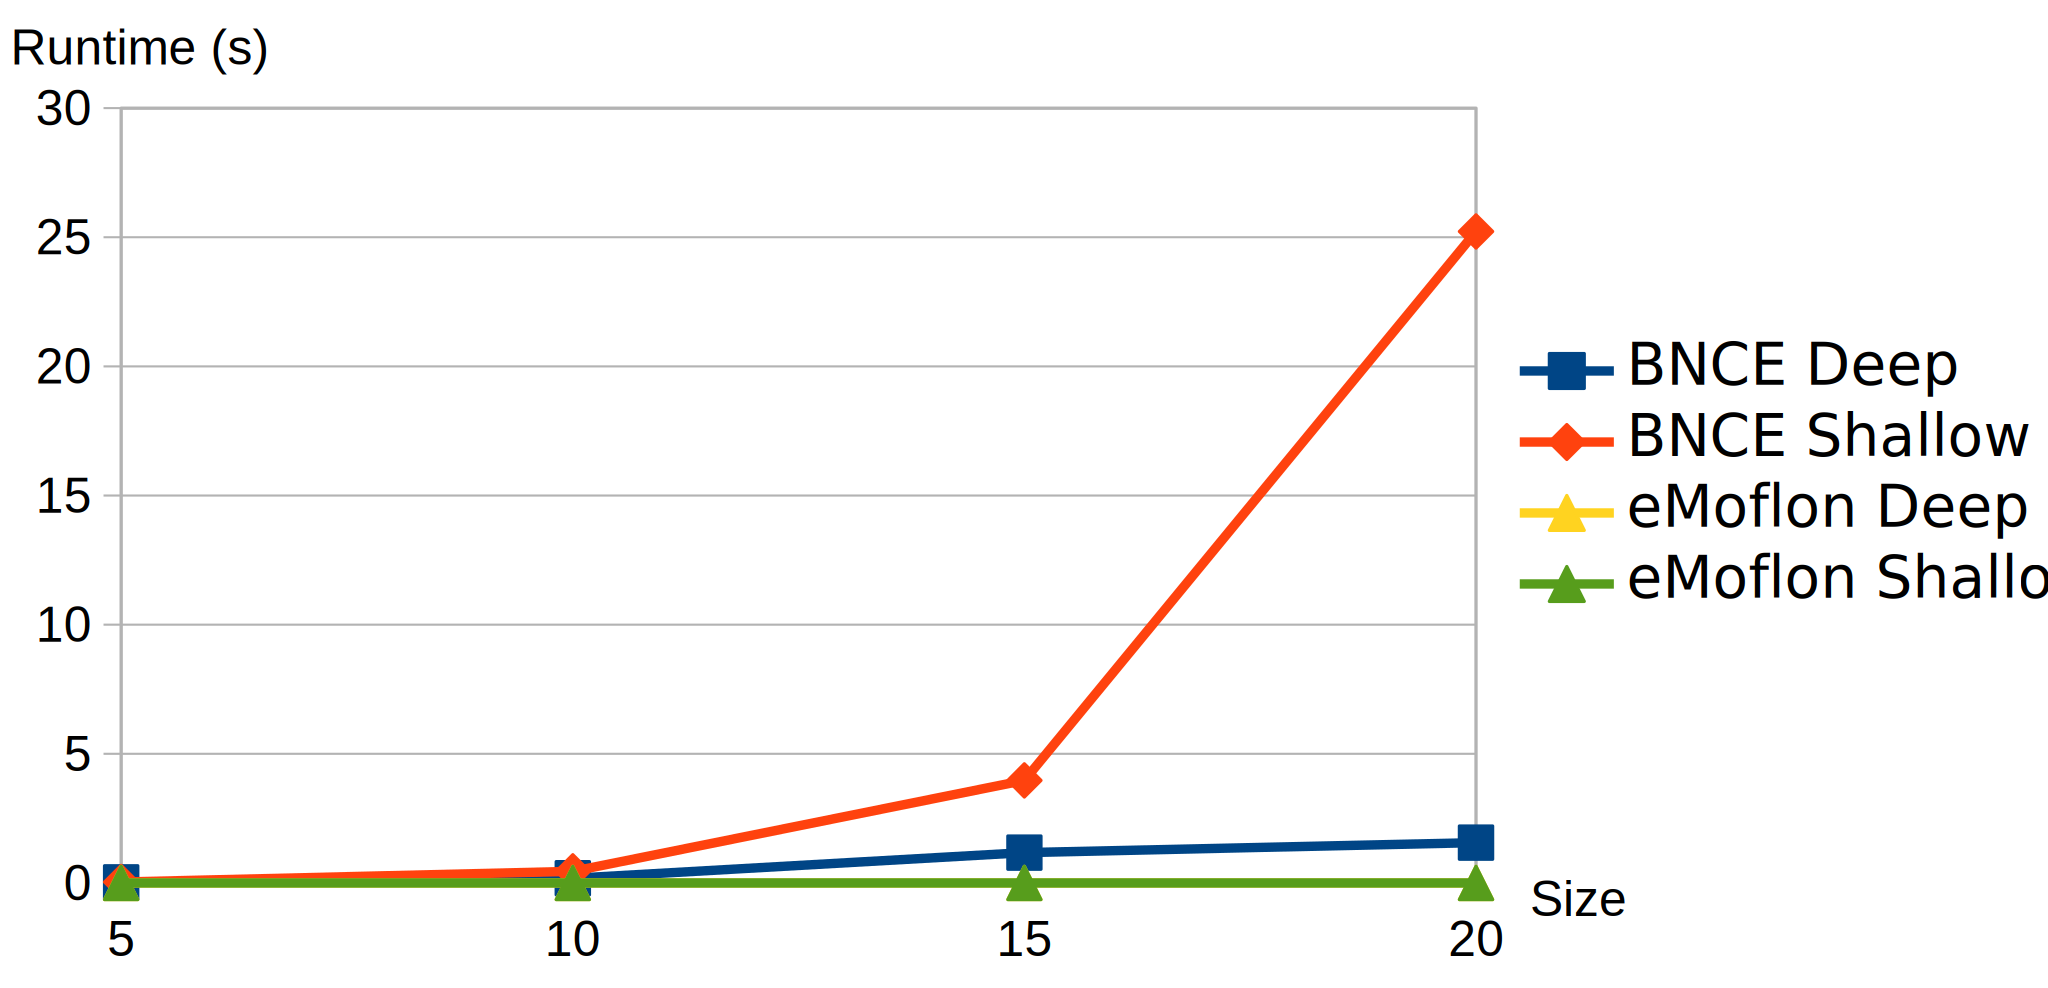
\includegraphics[width=\textwidth]{figures/performance/pseudocode2controlflow}
		\end{figure}
	\end{frame}
	
	%-------------------
	%  Conclusion
	%-------------------
	\section{Conclusion}
	\begin{frame}
		\frametitle{Conclusion}
		\tableofcontents[currentsection, currentsubsection] 
	\end{frame}
	
	\begin{frame}{Conclusion}
		\begin{itemize}
			\item New context-free TGG formalism
			\begin{itemize}
				\item Outperforms standard TGG in 2 evaluated cases and in average
				\item Special potential for code-generation
				\item Extension with positive application conditions
			\end{itemize}
			\pause
			\item Future Work
			\begin{itemize}
				\item Efficient transformer: Top-down parser
				\item Broader evaluation including empirical assessment with engineers and performance reports
				\item Model synchronization
			\end{itemize}
		\end{itemize}
	\end{frame}
	
	%-------------------
	% References
	%-------------------
	\section{References}
	\begin{frame}
		\frametitle{References}
		\tableofcontents[currentsection, currentsubsection] 
	\end{frame}
	
	\begin{frame}
		\frametitle{References}
		\tiny
		\bibliographystyle{plainnat}
		\bibliography{bibliography}
	\end{frame}

	%------------------------------------------------
	% Appendix
	%------------------------------------------------
	\appendix
	
	\begin{frame}{Appendix}
		\begin{center}
			{\LARGE \textbf{Appendix}}
		\end{center}
	\end{frame}

	\begin{frame}{Pseudocode to Controlflow -- Full}
		\begin{columns}
			\column{\dimexpr\paperwidth-20pt}
			\input{examples/pseudocode2controlflow-tgg-full-00}
		\end{columns}
	\end{frame}

	\begin{frame}{Pseudocode to Controlflow -- Full}
		\input{examples/pseudocode2controlflow-tgg-full-01}
	\end{frame}
	
	\begin{frame}{Class to Database -- Full}
		\begin{columns}
			\column{\dimexpr\paperwidth-20pt}
			\input{examples/class2database-tgg-full-00}
		\end{columns}
	\end{frame}
	
	\begin{frame}{Class to Database -- Full}
		\centering	
	\begin{tikzpicture}[grammar]
		\node[rid] at (\ridX,\ridY) {$r_5:$};
		\draw (\lhsX,0) node[lhs] (lhs) {SA ::=};
		%%
		\draw (0.5,0) node[t, label=90:$s_{50}$] (s1) {a};
		\draw (0.5,-1) node[nont, label=90:$s_{51}$] (s2) {SA};
		%%
		\draw (2,0) node[t] (c1) {ac};
		\draw (2,-1) node[nont] (c2) {SA};
		%%
		\draw (3.5,0) node[t, label=90:$t_{50}$] (t1) {co};
		\draw (3.5,-1) node[nont, label=90:$t_{51}$] (t2) {SA};
		%%
		\draw[morph] (c1) -- (s1);
		\draw[morph] (c1) -- (t1);
		\draw[morph] (c2) -- (s2);
		\draw[morph] (c2) -- (t2);
		%%%%
		\draw[pipe] (4,\pipeBY) -- (4,-1);
		%%
		\node[rid] at (4.7,\ridY) {$r_6:$};
		\draw (4.5,0) node[empty] (s3) {$\emptyTG$};
	\end{tikzpicture}
	%%%%%%%%%%%%%%%%%%%%%%%%%%%%%%%%%%%%%%%
	\vskip 5pt
	%%%%%%%%%%%%%%%%%%%%%%%%%%%%%%%%%%%%%%%
	\begin{tikzpicture}[grammar]
		\node[rid] at (\ridX,\ridY) {$r_7:$};
		\draw (\lhsX,0) node[lhs] (lhs) {A ::=};
		%%
		\draw (0.5,0) node[t, label=90:$s_{70}$] (s1) {a};
		\draw (0.2,-1) node[nont, label=90:$s_{71}$] (s2) {A};
		\draw (1,-0.7) node[pac, label=45:$s_{72}$] (s3) {c};
		\draw[pacedge] (s1) -- (s3) node [vredgeLabel] {$\psi$};
		%%
		\draw (2,0) node[t] (c1) {ac};
		\draw (2,-1) node[nont] (c2) {SA};
		\draw (2,-0.5) node[pac] (c3) {ct};
		%%
		\draw (3.5,0) node[t, label=90:$t_{70}$] (t1) {co};
		\draw (3.8,-1) node[nont, label=90:$t_{71}$] (t2) {A};
		\draw (3,-0.7) node[pac, label=135:$t_{72}$] (t3) {t};
		\draw[pacedge] (t1) -- (t3) node [vledgeLabel] {$\delta$};
		%%
		\draw[morph] (c1) -- (s1);
		\draw[morph] (c1) -- (t1);
		\draw[morph] (c2) -- (s2);
		\draw[morph] (c2) -- (t2);
		\draw[morph] (c3) -- (s3);
		\draw[morph] (c3) -- (t3);
		%%%%
		\draw[pipe] (4.4,\pipeBY) -- (4.4,-1);
		%%
		\node[rid] at (5.1,\ridY) {$r_8:$};
		\draw (5,0) node[empty] (s3) {$\emptyTG$};
	\end{tikzpicture}

	\end{frame}

	\begin{frame}{Performance Evaluation}
		\begin{itemize}
			\item \emph{Star} to \emph{Wheel}
		\end{itemize}
		\begin{figure}
			\centering
			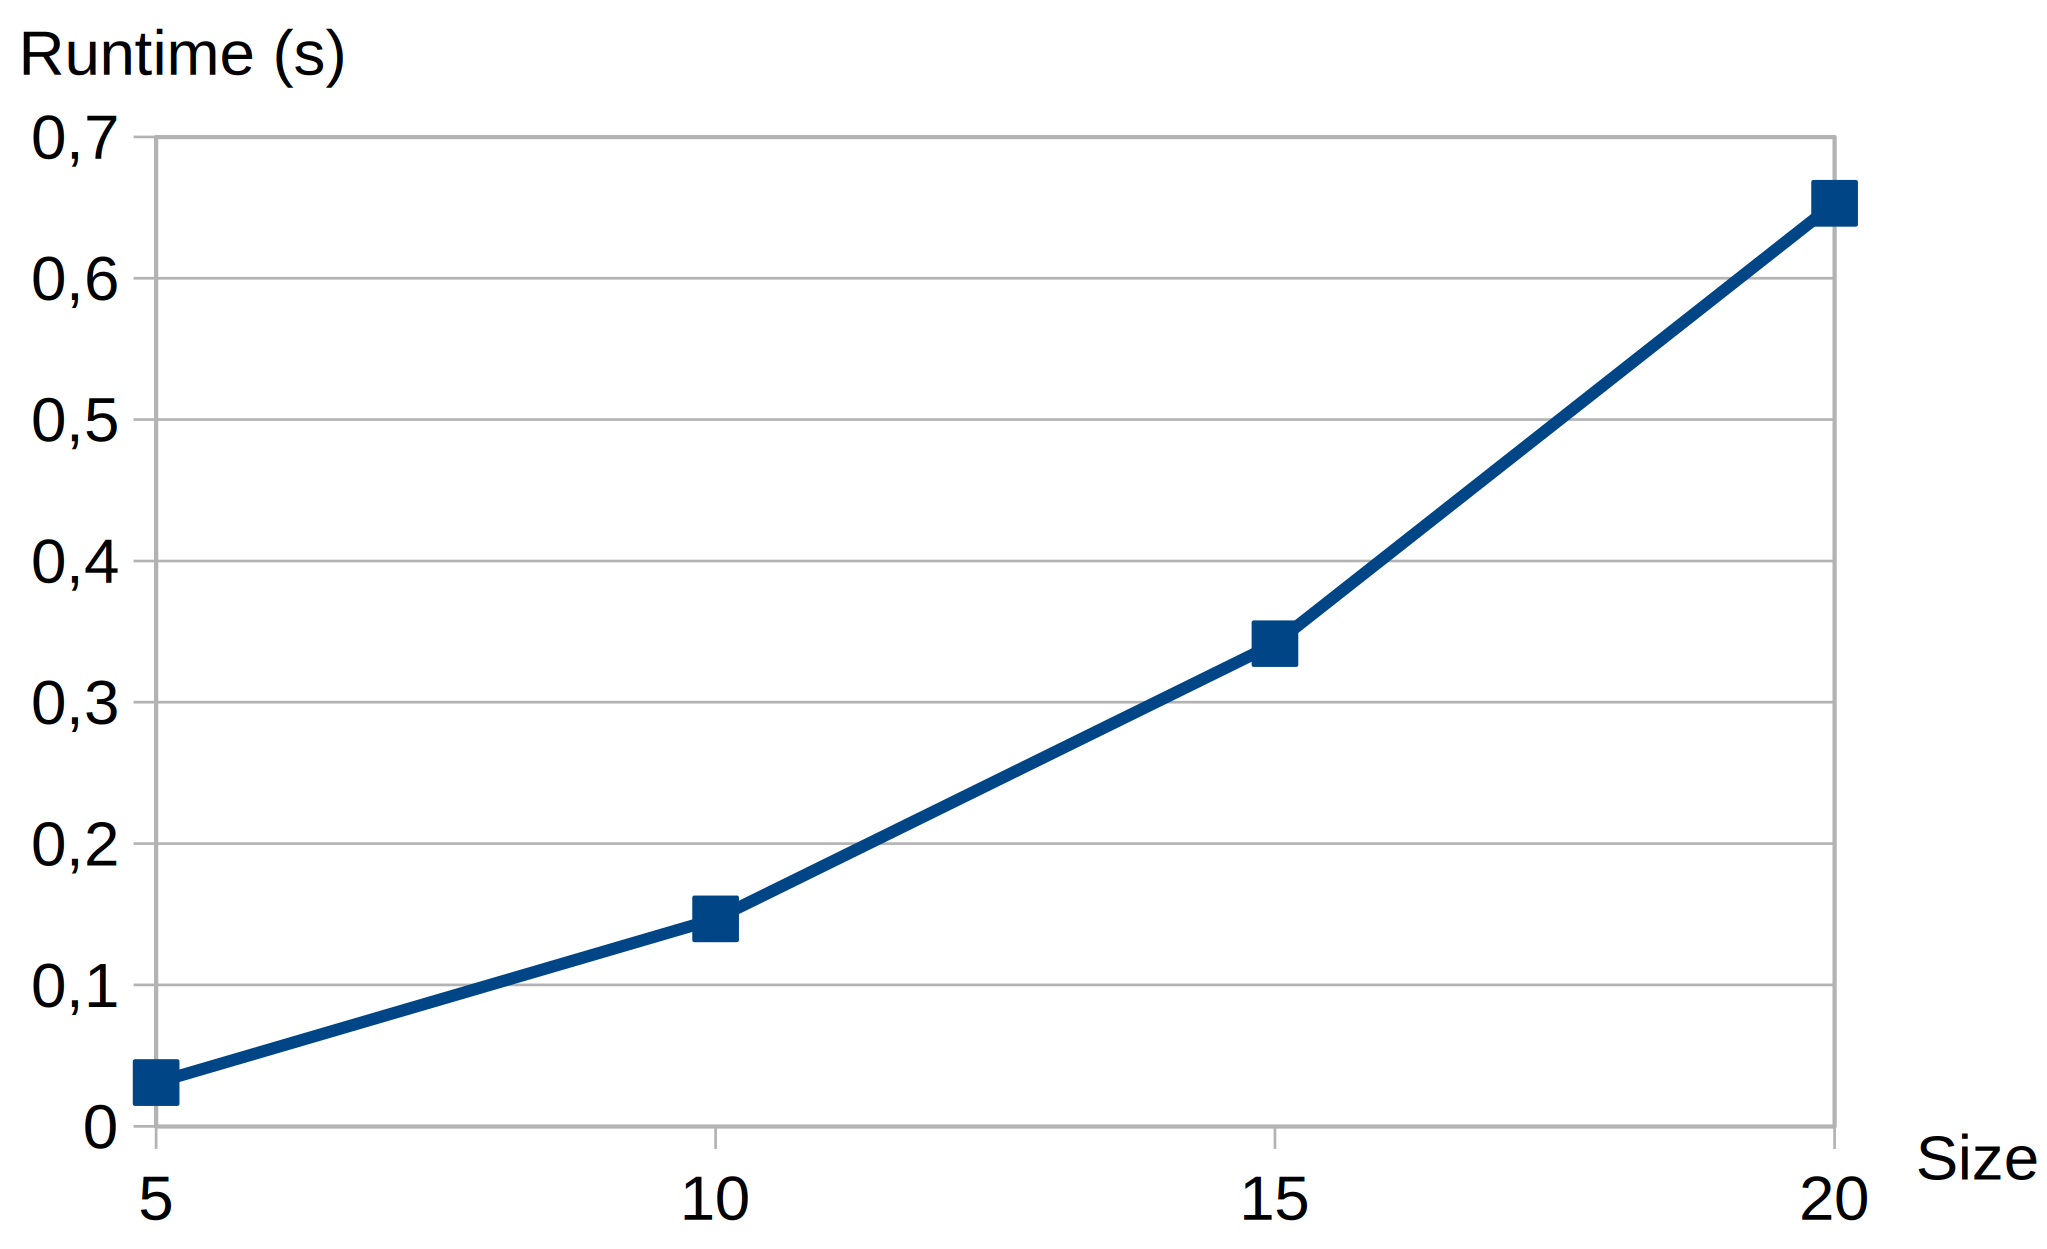
\includegraphics[width=\textwidth]{figures/performance/star2wheel}
		\end{figure}
	\end{frame}
	
	\begin{frame}{Performance Evaluation}
		\begin{itemize}
			\item \emph{BTree} to \emph{XBTree}
		\end{itemize}
		\begin{figure}
			\centering
			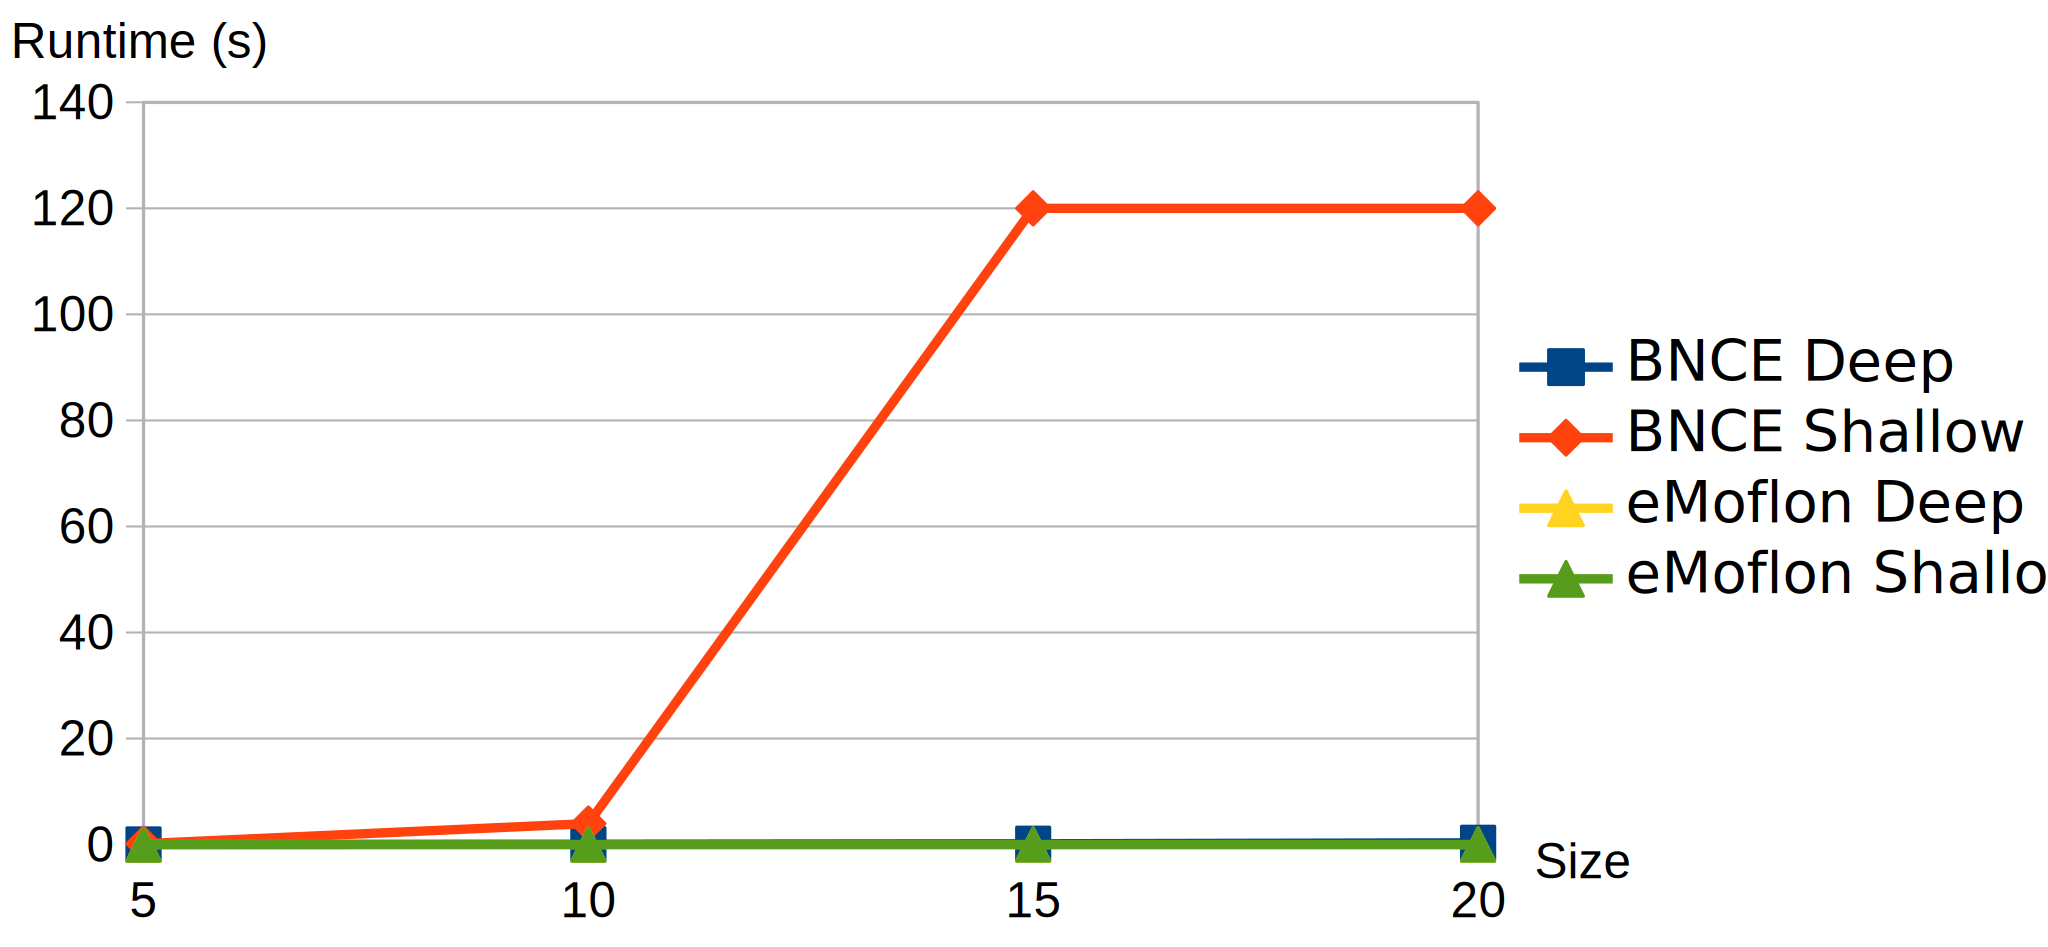
\includegraphics[width=\textwidth]{figures/performance/btree2xbtree}
		\end{figure}
	\end{frame}
	
	\begin{frame}{Performance Evaluation}
		\begin{itemize}
			\item \emph{StateMachine} to \emph{PetriNet}
		\end{itemize}
		\begin{figure}
			\centering
			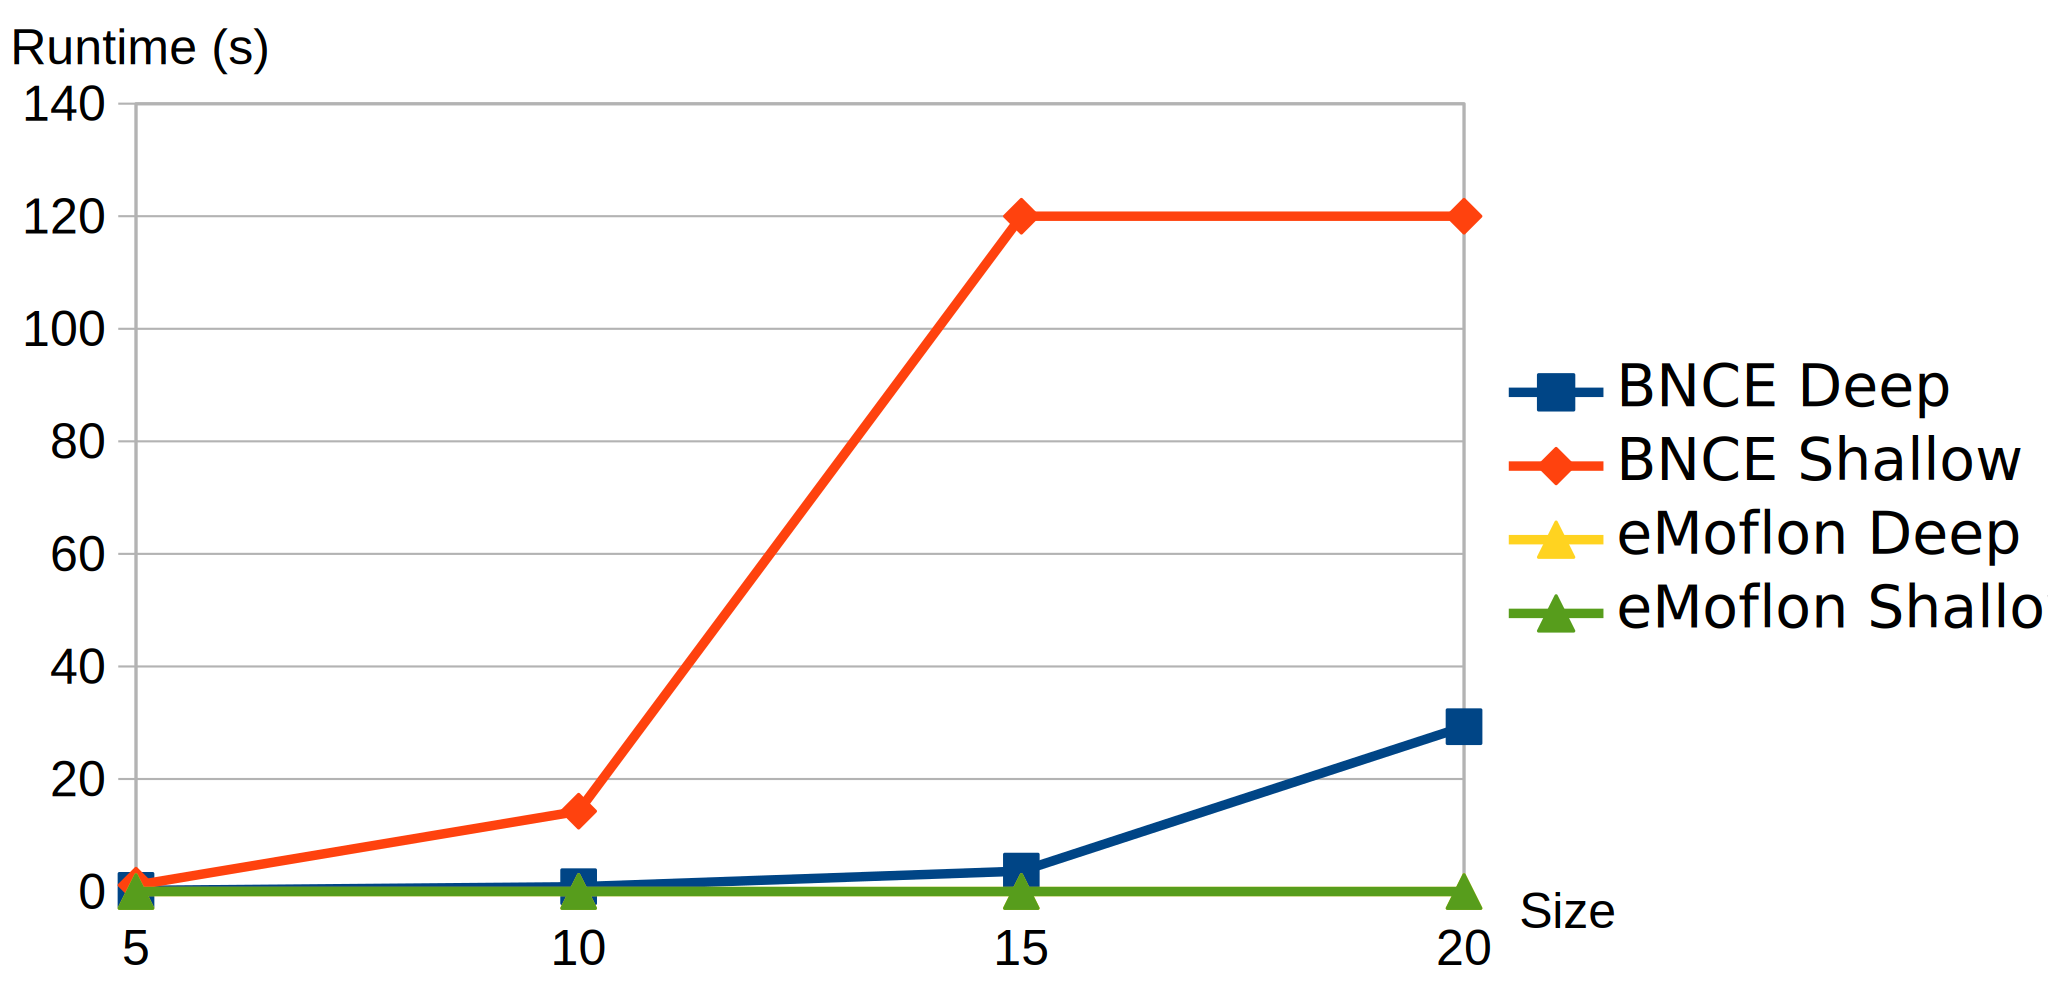
\includegraphics[width=\textwidth]{figures/performance/statemachine2petrinet}
		\end{figure}
	\end{frame}
	
	\begin{frame}{Performance Evaluation}
		\begin{itemize}
			\item \emph{Class} to \emph{Database}
		\end{itemize}
		\begin{figure}
			\centering
			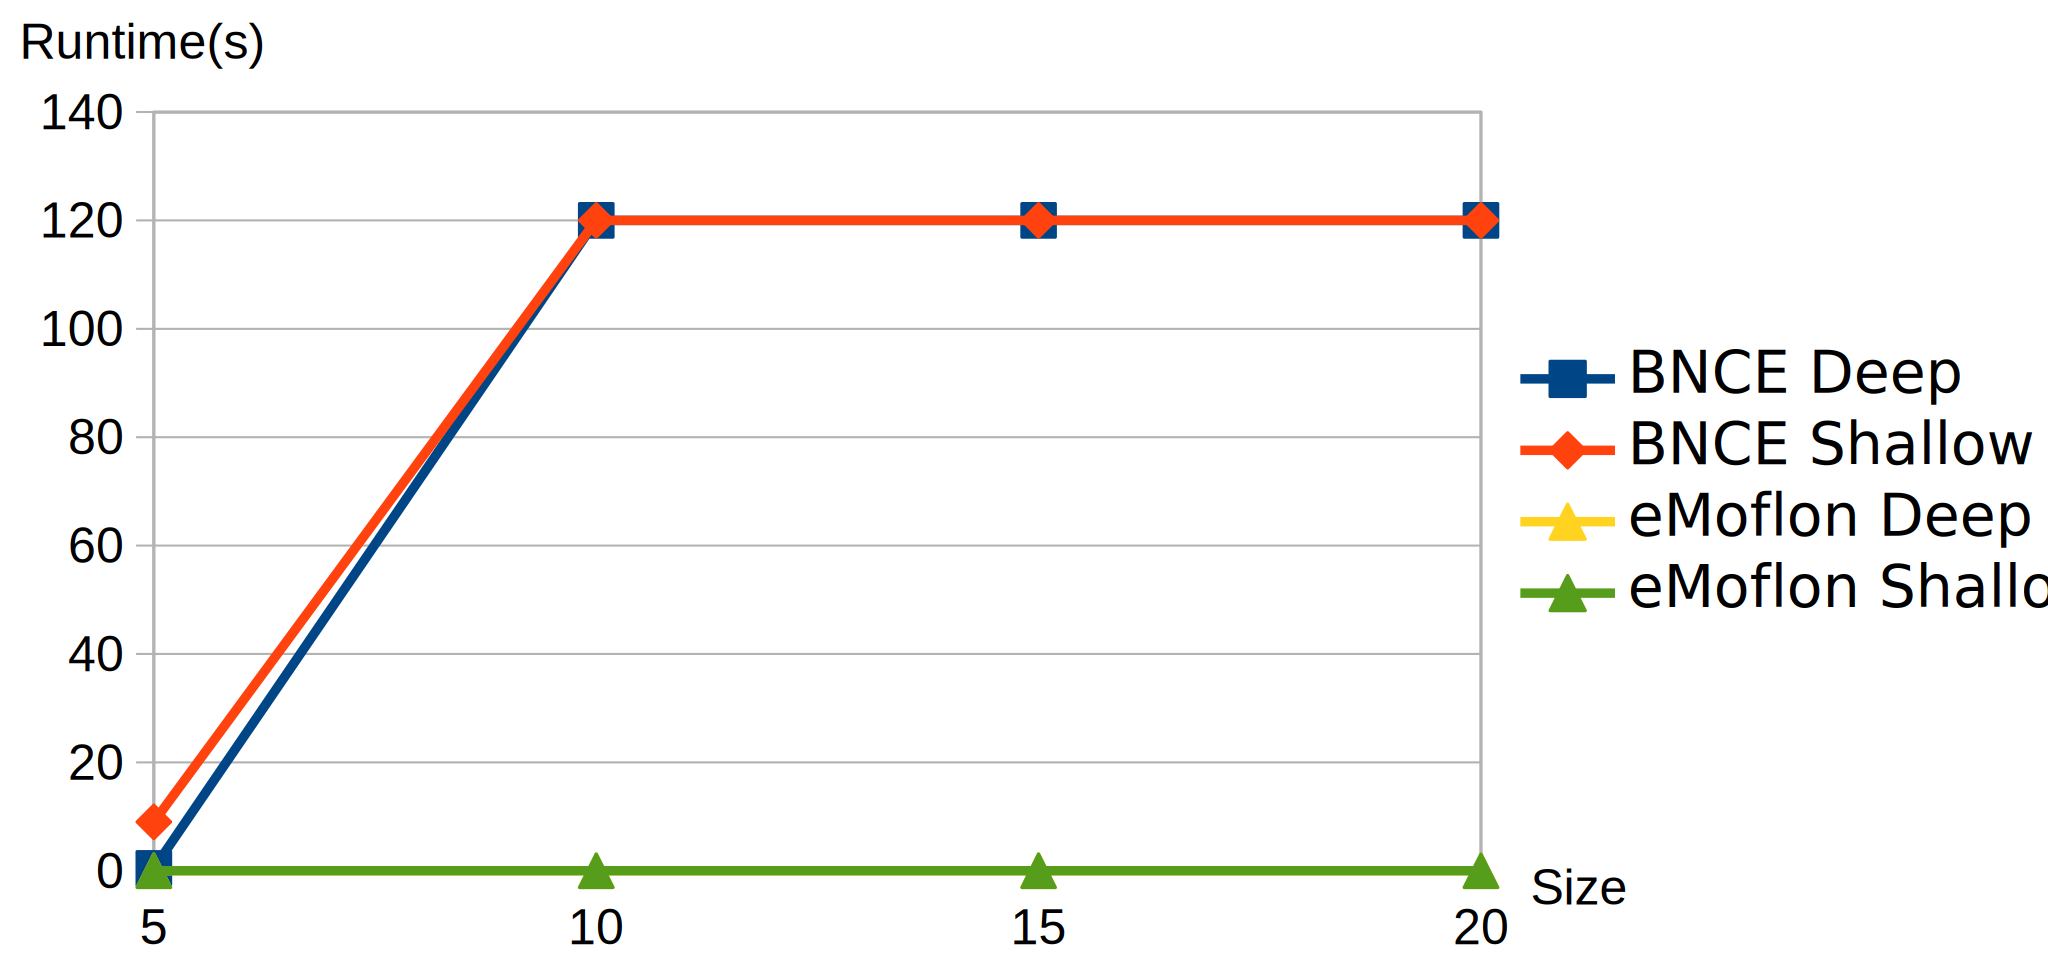
\includegraphics[width=\textwidth]{figures/performance/class2database}
		\end{figure}
	\end{frame}

\end{document}
